%!TEX root = mb.tex


\section{Introduction}\label{sec:intro}


    Network processing appliances (``middleboxes'') such as firewalls, proxies, and intrusion detection systems are crucial components of modern networks~\cite{aplomb}. 
     In recent trends, more and more organizations {\it outsource} their network processing, either to cloud providers~\cite{aplomb, aryaka, zscalar} or to service providers through Network Functions Virtualization (NFV)~\cite{nfv}. This strategy promises to reduce costs, decrease the burden of managing and configuring these devices, and provide elasticity and fault tolerance, as documented in~\cite{aplomb}.
Already now, the NFV working group~\cite{nfvwg} has over 250 members ranging from large telecoms to hardware manufacturers, all of whom are investing in new technologies to enable outsourced traffic processing.
   
   Nevertheless, outsourcing middleboxes to the cloud brings a new and important challenge: the privacy of the traffic. The cloud provider now receives  the organization's traffic to examine it and run middlebox functionality, but as a consequence it sees the {\em unencrypted} traffic. This means that the cloud has access to potentially sensitive packet payloads,  IP addresses, and ports revealing private or confidential information about the organization. This situation is worrisome considering the amount of documented data breaches by cloud employees or hackers breaking into clouds~\cite{XXX}.
   Hence, in this paper, we ask: is it possible to enable a third party to perform traffic processing for an enterprise, {\em without seeing the enterprise's traffic}?
   
   
   

% Justine's text unchanged: (the above is a combination of Justine & Raluca)
%    Network processing appliances (''middleboxes'') such as firewalls, proxies, and intrusion detection systems make up a substantial fraction of modern network infrastructure; studies show that as much as 1/3 of enterprise network hardware consists of such devices~\cite{aplomb}.
%    However, recent trends suggest that this fraction may begin to decline as more and more networks begin to {\it outsource} their network processing, either to cloud providers~\cite{aplomb, aryaka, zscalar} or to service providers through Network Functions Virtualization (NFV)~\cite{nfv}.
%    At the time of this writing, the NFV working group~\cite{nfvwg} has over 250 members ranging from large telecoms to hardware manufacturers, all of whom are investing in new technologies to enable outsourced traffic processing.
%    For consumers, outsourcing traffic processing offers many of the same benefits that outsourcing compute and storage have attained through cloud computing: decreased costs, ease of management, the ability to scale and failover on demand, \etc{}.
%    Nevertheless, outsourcing network processing brings new challenges, and among them, an issue which is critical to most enterprises: privacy.
%    
%    Under traditional middlebox deployments, traffic is processed and inspected by devices which are owned, hosted, and managed entirely within the enterprise itself.
%    Encrypted traffic is often decrypted to enable deep packet inspection (DPI) such as intrusion detection and exfiltration detection.
%    This configuration places critical trust in the hands of network administrators, who can potentially read or even modify {\it any} connection within the company.
%    Outsourcing shifts this trust away from network administrators who are employed and monitored by the company whose data is being processed, and to a third party company with its own employees, hiring practices, and motivations.
%    Hence, in this paper, we ask: is it possible to enable a third party to perform traffic processing for an enterprise, without transferring the ability to read and monitor the enterprise's traffic?
%    
% 
     
     \qu{service provider or cloud? change in title, text and figures}
     
     
  
    We design and build \sys (read ``embark"), the first system that enables running middleboxes at a cloud provider while maintaining the privacy of the traffic against an attacker with access to all cloud data.  \sys's name concatenates the words MB (middlebox) and Ark (protection). \sys supports a wide range of middleboxes, in fact, all middleboxes documented in~\cite{aplomb} to fit in the cloud outsourcing model. These are: firewall, NAT, intrusion detection systems (IDS), data exfiltration systems, web proxy, load balancing and VPN. \sys supports these applications with competitive performance. 
    
    The approach in \sys is to send encrypted traffic to the middleboxes in the cloud and have the cloud process encrypted traffic without ever decrypting it. \sys encrypts the packet payload as well as information in the header (IP addresses, ports). Since the cloud receives only encrypted traffic and no decryption key, it cannot see the private data. However, making such approach in a practical way for the wide-range of middlebox applications is challenging and requires a set of new techniques.
    
    
    
    
\begin{table}[t!]
\centering
\begin{tabular}{p{3.2cm}|p{2.9cm}|p{1cm}}
{\bf Application}  & {\bf Operations used} & {\bf Details} \\
\hline \hline
IP Firewall &   range  & \S\ref{sec:firewall} \\
Application Firewall & range, keyword  & \S\ref{sec:firewall}\\
NAT & range  & \S\ref{sec:nat} \\
IP Forwarding  & \textcolor{red}{XXX} &  \textcolor{red}{XXX} \\
Load Balancer L4 & range & \S\ref{sec:loadb}\\
Load Balancer L7  & range & \S\ref{sec:loadb}\\
Web Proxy/Cache  & keyword & \S\ref{sec:proxy}\\
Intrusion Detect (IDS)  & range, keyword & \S\ref{sec:IDS}\\
Data Exfiltration  & keyword & \S\ref{sec:IDS} \\
VPN Gateway &  none & \S\ref{sec:vpn} \\ 
\end{tabular}
\caption{Middlebox applications supported by \sys and the type of match it needs to perform. Each application is further described in the section specified. \label{tab:apps} }
\end{table}


\begin{figure*}[t!]
\centering
\subfigure[Enterprise to external site communication]{
  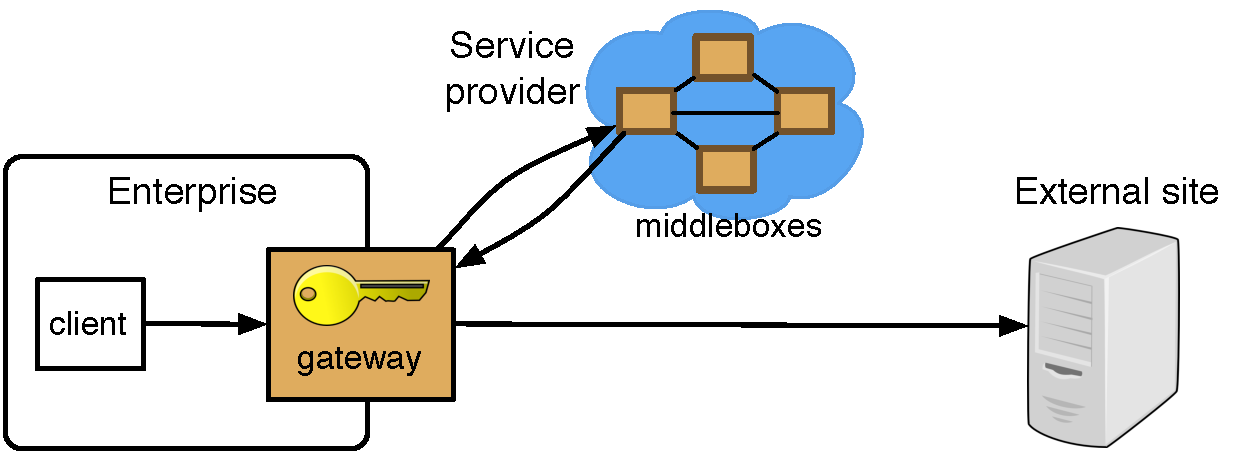
\includegraphics[width=3.3in]{fig/model_1.pdf}
  \label{fig:model1} }
%
\hfill  
\subfigure[Enterprise to enterprise communication]{
   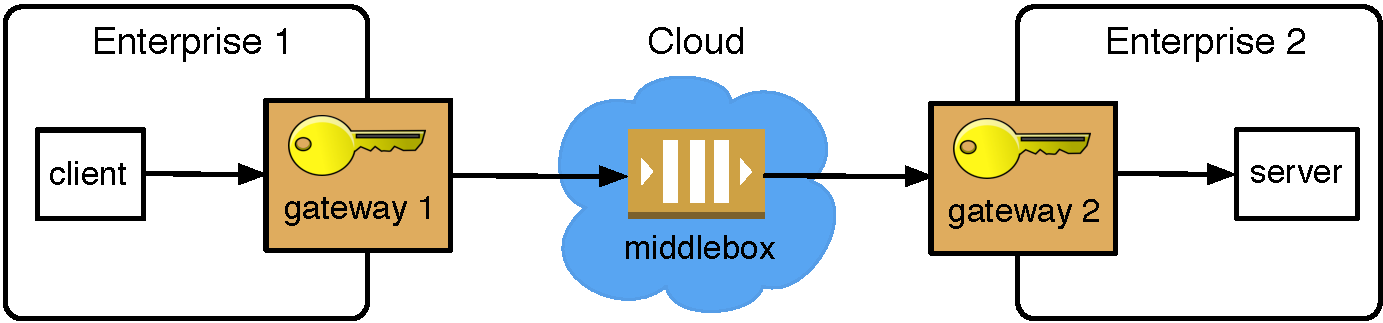
\includegraphics[width=3.1in]{fig/model_2.pdf}
     \label{fig:model2}}
     
     %
\caption{System architecture. Aplomb and NFV system setup with \sys encryption  at the gateway. \label{fig:sys-overview}}
\end{figure*}

    \subsection{Challenges, techniques, and contributions}
    
The first challenge is that performing generic computation on encrypted data is prohibitively practical. The applications we are trying to support provide complex functionalities. For example, firewall and NAT examine packet header information such as IP address and ports; for IDS and data exfiltration detection, the middlebox (MB) examines packet payload and tries to match complex rules (keyword matching, offset information, some regular expressions, etc). The existing generic homomorphic encryption schemes are many orders of magnitude impractical~\cite{aesFHE}.

Fortunately, recently, there has been a new vision for building practical such systems, as in CryptDB~\cite{cryptdb}, and we follow this vision too. Instead of aiming for generic computation, the idea is to identify core operations that underlye the functionality in the system and to support each with a fast specialized encryption scheme. Unfortunately, neither the core operations nor the encryption schemes in CryptDB fit in our network setting so we need to start from zero.

We study the relevant middlebox applications, and we managed to identify two core operations that underlie all these middleboxes: {\em keyword match} and {\em range match}. Keyword match (KW match) refers to  identifying if a keyword appears in a byte stream at some offset. There are two types of keyword match: regular and cross-boundary. Since we are dealing with network packets, a keyword may appear across two different packets (e.g., ``alice'' appears at the boundary of the packets ``I see ali'' and ``ce at the zoo''.). For example, keyword match is useful for data exfiltration when a watermark is searched for in the traffic, for IDS when malicious strings are seached on the traffic and for web proxy when a file id to be retrieved from the cache is identified. 
Range match refers to when a value $x$ matches an interval of two values ($x_1$ and $x_2$). Range match is useful to encrypt ports and IP addresses in firewall rules, for example, when the firewall needs to drop traffic in from a certain IP prefix (which can be seen as an interval of IP addresses). Note that range match supports a basic version of KW match, complete equality check. 

Table~\ref{fig:apps_ops} summarizes the middleboxes we support and the operations they rely on. 





\begin{itemize}

\item how to secure (which information need to protect)
\item how does mbark work: building blocks, applications secured (a nice table could go well here)
\item perhaps aplomb overview figure already in intro
\item contribution
\end{itemize}

\subsection{Implementation and evaluation}
